%!TEX root = ../../dissertation.tex
%%%%%%%%%%%%%%%%%%%%%%%%%%%%%%%%%%%%%%%%%%%%%%%%%%%%%%%%%%%%%%%%%%%%%%%%%%%%%%%%
\section{Evaluation Methodology}
\label{c4:methodology}

With the mobile network load defined and possible influencing factors described, we now move on to apply these to an actual mobile network. For this data from passive network traces will be employed. But first, the monitoring setup and the captured has to be described in this section. This also includes a description of some methods required to examine specific device types and other device-based factors from the dataset.

While this chapter only employs passive measaurements, Chapter~\ref{chap:mobilestreaming} will additionaly deal with approaches to conduct meaningful active device-based measurements and additionally set up a simulation/emulation testbed based on the results.

%%%%%%%%%%%%%%%%%%%%%%%%%%%%%%%%%%%%%%%%%%%%%%%%%%%%%%%%%%%%%%%%%%%%%%%%%%%%%%%%
\subsection{Network and Monitoring Setup}

For our analysis, the \gls{METAWIN} monitoring system developed in a previous third-party research project and deployed in the network of an Austrian mobile operator is used. \cite{ricciato_2011,ricciato2006traffic}


\begin{figure}[htb]
	\centering
	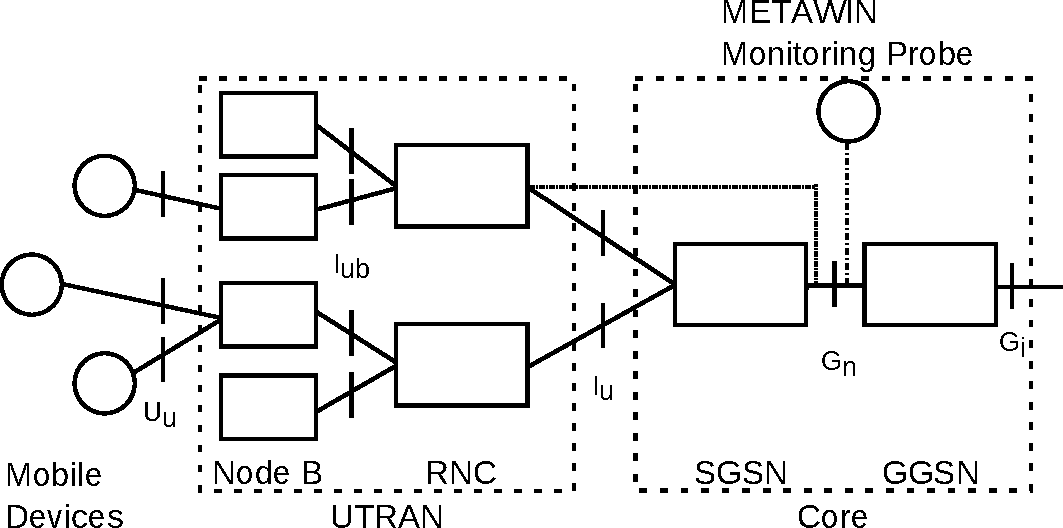
\includegraphics[width=1.0\textwidth]{images/umts-network.pdf}
	\caption{Location of the \acrshort{METAWIN} monitoring probe in the \gls{3G} core network}
	\label{c4:fig:umtsnetwork}
\end{figure}



The measurement taps are located at the Gn interface at one \gls{GGSN} within the core network as depicted in Figure~\ref{c4:fig:umtsnetwork}. It gives access to a wide spectrum of core \gls{gtp} signaling, including the mobility and tunnel management. \cite{3gpp.29.060}. The system does not offer a complete packet trace, but aggregates every signaling transaction and user traffic flow down to a number of select fields. This includes \gls{gtp} \gls{IE} such as the \gls{RAT}  as well as the terminal types of the mobile clients. The latter is determinable by the \gls{TAC} part of the \gls{IMEI} (cf.~\cite{3gpp.23.003}) and will be discussed later in detail.

In the network under study, a direct tunnel setup might be used for \gls{UMTS}-using \glspl{UE} consisting of a direct link between \glspl{GGSN} and the \glspl{RNC} and circumventing the \gls{SGSN}. It is only used for transporting user-plane traffic, signaling procedures are carried out in the normal way between \glspl{SGSN} and \gls{GGSN}. Therefore, only the Gn interface at \gls{GGSN} is seeing the complete core network traffic, explaining the location of the tap.


Recording data in a live network necessitates meeting strict privacy requirements regarding the handling of user-related data. \gls{METAWIN} complies with this by anonymizing all user-identifying. Application-level payload is removed and all user identifiers (e.g. \gls{IMSI}) are non-reversibly hashed before recording. \glspl{UE} in a dataset can still be differentiated by the hashes but not traced back to the actual user. The wiretaps deployed within the monitoring system are time-synchronized with \gls{GPS}. Accordingly, the packet timestamps have an accuracy of $\pm100$ ns or better.
%~\cite[p.97-98]{donnelly_high_2002}.


%%%%%%%%%%%%%%%%%%%%%%%%%%%%%%%%%%%%%%%%%%%%%%%%%%%%%%%%%%%%%%%%%%%%%%%%%%%%%%%%
\subsection{Dataset Description}

%<--||

The \gls{METAWIN}-recorded dataset used in our evaluation is a week-long trace from the third week of April 2011. It consists of 2.2 billion aggregated flows for the user traffic and 410 million \gls{gtp} Tunnel Management transactions, the latter representing the data base for this paper. It was tapped at one of the \glspl{GGSN} of the operator, and contains about half of the total traffic volume handled by the operator in this period. The \gls{gtp} data contains the response codes for each transactions. With these codes, failed interactions can be sorted out and treated separately.

We fed the records into a SQL database, and conducted further evaluations through scripted queries on the database. Any privacy-relevant data, e.g. the \gls{IMEI}, \gls{MS-ID} and any IP address involved, is only visible as hashes and is processed in a privacy-preserving manner.  Since the hashing of the \gls{IMEI} is consistent throughout the dataset, user traffic flows and the \gls{gtp} data can be cross-correlated despite anonymization, giving the opportunity for further research.


In order to evaluate our models, we use data gathered from a nation-wide mobile operator. This allows for precise core network evaluations and the creation statistical fits for the observed processes.
In this section we first describe the dataset used for the evaluation and afterwards we derive the random variables required for our models.

 For this investigation we exclusively use \gls{gtp} protocol data gathered by \gls{METAWIN}. This includes the \gls{RAT} identifier as well as the terminal types of the mobile clients, by use of the \gls{TAC} part of the \gls{IMEI}. % \cite{etsi_3gpp_2008} for GTP on Gn
To meet privacy requirements, \gls{METAWIN} anonymizes all captured data. The application-level payload is removed and all user identifiers are hashed with one-way functions before recording. Individual \glspl{MS} in our dataset can be differentiated by the hashed \gls{MS-ID}, but not traced back to the actual user.

The dataset used in our evaluation is a week-long trace from the third week of April 2011. It consists of $2.2$ billion aggregated flows for the user traffic and $410$ million \gls{gtp} Tunnel Management transactions. It was tapped at one of the \glspl{GGSN} of the operator, and contains about half of the total traffic volume handled by the operator in this period.
%The records were stored in a SQL database, with most of the statistical evaluation conducted using R.

Our dataset, kindly provided by a nation-wide mobile operator and recorded using the \gls{METAWIN} monitoring system, was taken in the third week of April 2011. It consists of seven days of aggregated flow-level data for the user traffic and a summary entry for every \gls{gtp} Tunnel Management transaction, the latter representing the data base for this paper. It was tapped at one of the \glspl{GGSN} of the operator, and contains about half of the total traffic volume handled by the operator in this period. The \gls{gtp} data contain the response codes for each transactions. With these codes, failed interactions can be sorted out and treated separately.

We fed the records into a SQL database, and conducted further evaluations through scripted queries on the database. Any privacy-relevant data, e.g. the \gls{IMEI}, \gls{MS-ID} and any IP address involved, is only visible as hashes and can only be processed in anonymized form. Individual device types can be identified in form of the unhashed \gls{TAC} on every entry. Since the hashing of the \gls{IMEI} is consistent, user traffic flows and the \gls{gtp} data can be cross-correlated despite anonymization, giving the opportunity for further research.

%%%%%%%%%%%%%%%%%%%%%%%%%%%%%%%%%%%%%%%%%%%%%%%%%%%%%%%%%%%%%%%%%%%%%%%%%%%%%%%
\subsection{Device Identification}

Individual device types can also still be identified in form of the \gls{TAC} on every entry. The \gls{TAC} is part of the \gls{IMEI}, uniquely identifying each device type \cite{3gpp.23.003}. The rest of the \gls{IMEI} constitutes the serial number of the involved devices, which is not present in the data.

In our dataset, the \gls{TAC} field is provided in clear\-text, whereas the \gls{IMEI} is only available in hashed form to preserve the privacy of device owners. The \gls{TAC} is contained in the first eight decimal digits of the \gls{IMEI}, uniquely identifying each device type \cite{3gpp.23.003}. The rest of the \gls{IMEI} constitutes the serial number of the involved devices.

\glspl{TAC} are managed by the \gls{GSMA} which in turn assigns local organizations, distinguished by the first two digits of the \gls{TAC} as Reporting Body Identifier, to allocate \glspl{TAC} to manufacturers. However, this allocation information is not freely available. Commercial databases exist, but this is neither affordable for research institutions, nor is it conducive to our goal of providing information to the public. While there are some websites that allow one to query for specific \glspl{TAC} for non-commercial purposes, only very few efforts attempt to collect \gls{TAC} information into a publicly available database. We based our data-mining efforts on a publicly available set\footnote{\url{http://www.mulliner.org/tacdb/}, Mulliner, C.}, with some additional devices collected on our own. Since the unit identification part of the \gls{IMEI} is just six decimal digits long, popular devices will even be assigned more than one TAC, making the acquisition of all relevant \glspl{TAC} even more complicated.

For our investigation, we went through large portions of the \glspl{TAC} present in our dataset, and identified and categorized the most important entries. In this case, importance means various metrics like the traffic volume, the number of flows, and the number of \gls{gtp} signaling messages for each \gls{TAC}. 


%%%%%%%%%%%%%%%%%%%%%%%%%%%%%%%%%%%%%%%%%%%%%%%%%%%%%%%%%%%%%%%%%%%%%%%%%%%%%%%%
\subsection{Device Classification}

For our investigation, we went through large portions of the \glspl{TAC} present in our dataset, and identified and categorized the most important entries. In this case, importance means various metrics like the traffic volume, the number of flows, and the number of \gls{gtp} signaling messages for each \gls{TAC}. 


After having available the device names for most \glspl{TAC}, we were able to add meta-information and categorize the entries based on their device type and operating system. For the device type we partitioned the devices roughly into smartphones, regular mobile phones and 3G USB dongles or 3G/WiFi routers. The operating system includes most of the popular incarnations found in the network at measurement time, including Android, iOS, and Symbian. Note however that many devices, especially USB dongles cannot be linked to any specific OS.


After having available the device names for most \glspl{TAC}, we were able to add meta-information to the entries in form of the following categories:

\begin{itemize}
\item The device type. We distinguished between smartphones, regular mobile phones and feature phones, and 3G USB dongles or 3G/WiFi routers.

\item The operating system of the device (if known), such as Android, iOS, Series 40, BlackBerry OS etc. This is especially interesting to identify potential differences in the core network signaling patterns of devices. Note however that we cannot link USB dongles and OS types from the \gls{TAC}.

\end{itemize}

\todo{extend this section}

%%%%%%%%%%%%%%%%%%%%%%%%%%%%%%%%%%%%%%%%%%%%%%%%%%%%%%%%%%%%%%%%%%%%%%%%%%%%%%%%
\subsection{TAC Statistics and Evaluation Validity}

It is important to know whether our \gls{TAC} mappings provide sufficient useful data to allow for the envisioned device discriminating statistics. Therefore, Table~\ref{c4:tbl:tacstats} provides some statistics on our knowledge of devices in the dataset. About 80 percent of all distinct devices active could be identified. Looking at the total number of \gls{gtp} signaling messages, we see that we can determine the device name of over 90 percent.
The flow data shows an even clearer picture, as we can identify almost all of the devices involved.


After applying the categorization to the \glspl{TAC} we evaluate the device composition in the network. The two largest portions of devices are smartphones  and 3G dongles, while classic cell phones do not seem to play a major role anymore. 
%We see about twice as many Android as iOS devices, possibly attributed either to the contractual situation of the operator or the wider price range of Android devices.

%Regular phones have negligible user traffic despite still making up one tenth of the device fraction. 

Initially, one planned endeavor was to investigate possible peculiarities of business phone behavior, especially of those easily identifiable Blackberry OS phones, but the number of distinct Blackberry devices in the dataset is too low to draw conclusions of any significance.

One observation across all device types is that about 18 percent of all mobile devices have activated their mobile data service and have signaling traffic, but do not cause any use plane traffic.

The difference between 3G dongles and smartphones is also noteworthy. While the former cause large amounts of user plane traffic (compared to the device numbers), they are responsible for but a low number of core network signaling events and tunnels. This picture is reversed for smartphones.



\begin{table}
\centering
\caption{Relative \acrshort{TAC} Statistics.}
\label{c4:tbl:tacstats}
\begin{tabu}{|l|X[r]|}
\hline
& \textbf{Portion of devices with entry in TAC DB}\\ \hline
\# of Flows & 99.72\% \\
Ratio of Traffic & 99.97\%\\
\# of Tunnels & 87.57\% \\
\# of GTP Signaling Msgs & 90.95\% \\
\# of Distinct \glspl{MS-ID} & 80.93\%\\ \hline
\end{tabu}
\end{table}

As we are working with an incomplete \gls{TAC} database it is important to know whether our \gls{TAC} mappings provide sufficiently useful data to allow for the envisioned device discriminating statistics. Therefore, Table~\ref{c4:tbl:tacstats} provides some statistics on our knowledge of devices in the dataset. About 80 percent of all distinct and active devices could be identified. Looking at the total number of \gls{gtp} signaling messages, we see that we can determine the device name of over 90 percent. The flow data shows an even clearer picture, as we can identify almost all of the devices involved.

After applying the categorization to the \glspl{TAC} we evaluate the device composition in the network. The two largest portions of devices are smartphones and 3G dongles, while classic cell phones do not seem to play a major role in the packet-switched domain anymore. One observation across all device types is that about 14 percent of all mobile devices have activated their mobile data service and have signaling traffic, but do not cause any user plane traffic.

The difference between 3G dongles and smartphones is also noteworthy. While the former cause large amounts of user plane traffic (compared to the device numbers), they are responsible for but a few core network signaling events and tunnels. This picture is reversed for smartphones.

